
\noindent The \textit{operator prodtuct expansion} (OPE) for the stress-energy tensor of a conformal quantum field theory is derived from the general structure of radial quantization, and is the primary algebraic tool in conformal field theory, and will later be used to introduce the Virasoro algebra. \\

\noindent In the previous lecture(s), we have been building a conformal quantum field theory from classical theories using the path integral in Euclidean space with the $n$-point correlation functions defined by

\begin{equation}
\langle \mathcal{T} [\hat{\phi} (x_1) \dots \hat{\phi} (x_n) ] \rangle = \lim_{\beta \rightarrow \infty} \frac{\int \mathcal{D} \phi \, \phi (x_1) \dots \phi (x_n) e^{-S[\phi]}}{\int \mathcal{D} \phi \, e^{-S[\phi]}}.
\end{equation}

\noindent The choice of coordinate axis for ``time'' leads to a different time-ordering symbol, Ward identities, and Hilbert space of states. For example, in Cartesian coordinates $\beta \equiv y$, and our quantum system exists on an infinitely long one-dimensional line. In polar coordinates $\beta \equiv r$, and our quantum system exists on a circle. \\

\noindent There are several good reasons to quantize to a circle. One: IR divergences are avoided. Two: it is more physical, since a quantum system on a circle is preparable in the lab. Three: it is more mathematically interesting due to the diffeomorphisms of the circle $S^1$. \\

\noindent For these reasons, we work in polar coordinates 

\begin{equation}
(x,y) \rightarrow (r,\theta) = \left(\sqrt{x^2 + y^2}, \text{arctan}\left(\frac{y}{x}\right)\right).
\end{equation}

\noindent In polar coordinates, spacetime forms a cylinder, rather then a plane or sheet, and ``equal-time'' slices are referred to as ``equal-radius'', and we will have equal-radius commutators for observables. \\

\noindent Introduce the \textit{radial-ordering symbol}

\begin{equation}
\mathcal{R} [\hat{A}(z) \hat{B} (w) ] = \begin{pmatrix} \hat{A} (z) \hat{B} (w), \,\, |z| > |w| \\ \hat{B} (w) \hat{A} (z), \,\, |z| < |w| \end{pmatrix}.
\end{equation}

\noindent Note that we will often leave out the radial-ordering symbol, such that whenever we write the expectation value of a product of quantum field operators, unless noted otherwise, we mean the vacuum expectation value of the radial-ordering of the operators

\begin{equation}
\langle \hat{T} (z) \hat{A} (w) \rangle \equiv \bra{0} \mathcal{R} [ \hat{T} (z) \hat{A} (w) ] \ket{0}.
\end{equation}

\noindent Now to make sense of the \textit{equal-radius} commutators, in analogy to the equal-time integral $\int dx$, which integrates over the remaining three spatial degrees of freedom in the Ward identity, we replace this Cartesian integral with the polar, complex analog

\begin{equation}
\int dx \rightarrow \oint dz.
\end{equation}

\noindent This contour integral will be over products of operators $\hat{a} (z) \hat{b} (w) \dots$. \\

\noindent We want to build a ``conserved charge'' $\hat{A} = \oint dz \,\, \hat{a} (z)$ from these operators, and then use them to build equal-radius (equal-time) commutators like $[\hat{A}, \hat{b} (w) ]$. and $\hat{a}$. \\

\noindent Consider the following set of contours $C_1$ and $C_2$ in the complex plane surrounding the point $w=x+iy$ by a distance $\epsilon$, the radius of the enclosed contour $W$.

\begin{figure}[H]
	\centering
	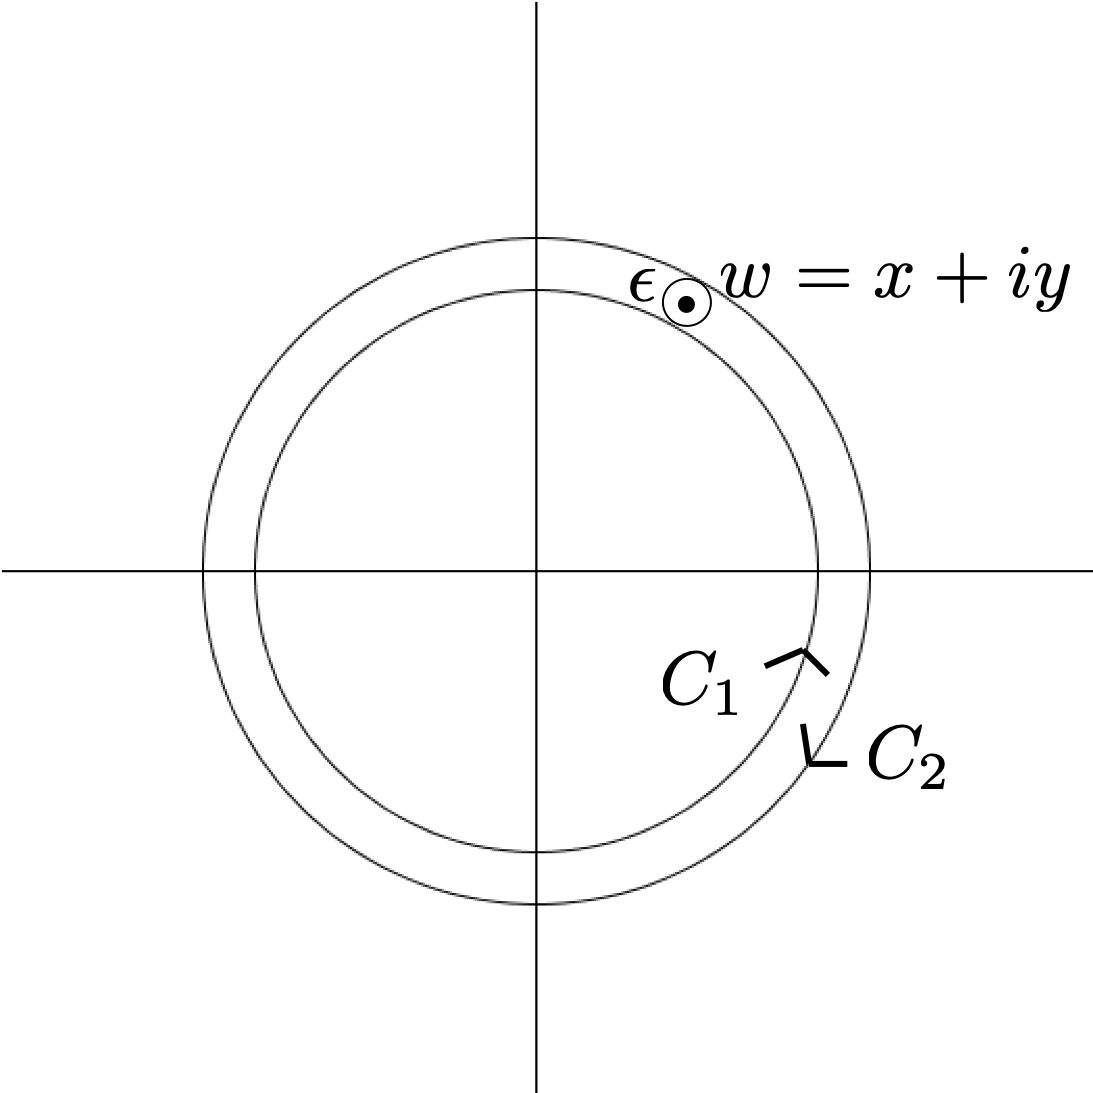
\includegraphics[width=2in]{images/radial_quant_contour.png} 
\end{figure} 

\noindent So, the commutator above can be written, assuming everything is holomorphic and nice,

\begin{align}
[ \hat{A}, \hat{b} (w)] &= \oint_W dz \,\, \hat{a} (z) \hat{b} (w) \\
&= \oint_{C_1} dz \,\, \hat{a} (z) \hat{b} (w) - \oint_{C_2} dz \,\, \hat{b} (w) \hat{a} (z).
\end{align}

\noindent Graphically, we can represent this as

%\begin{figure}[H]
%	\centering
%	\includegraphics[width=3in]{images/contour_commutator.png}
%\end{figure}

\noindent Remember that expressions such as $\hat{a} (z) \hat{b} (w) \dots = \hat{c} (z) \hat{d} (w) \dots$ are valid only within evacuum xpectation values with radial ordering of the arguments. \\

\noindent Now, apply this to primary fields of a conformal field theory, and let $\hat{\phi} (w, \bar{w})$ be a primary field and vary the field with respect to an infinitesimal conformal transformation, which gives us the conformal Ward identity (which must obey the differential equation for the infinitesimal conformal transformation $(\eta_{\mu\nu} \Box + (d-2) \partial_\mu \partial_\nu) (\partial \cdot \epsilon) = 0$).

\begin{align}
\delta_{\epsilon, \bar{\epsilon}} \hat{\phi} (w,\bar{w}) &= \frac{1}{2\pi i} \left( \oint dz \, \epsilon(z) \mathcal{R} [ \hat{T} (z) \hat{\phi} (w, \bar{w}) ] + \oint d\bar{z} \, \bar{\epsilon} (\bar{z}) \mathcal{R} [ \hat{\bar{T}} (\bar{z}) \hat{\phi} (w, \bar{w})] \right) \\
&= \frac{1}{2\pi i} \left( \oint_{C_1} dz \, \epsilon(z) \mathcal{R} [ \hat{T} (z) \hat{\phi} (w, \bar{w}) ] - \oint_{C_2} d\bar{z} \, \bar{\epsilon} (\bar{z}) \mathcal{R} [ \hat{\bar{T}} (\bar{z}) \hat{\phi} (w, \bar{w})] \right) \\
&= \frac{1}{2\pi i} \left( \oint dz \, \epsilon (z) [\hat{T} (z), \hat{\phi} (w,\bar{w})] + \oint d\bar{z} \, \bar{\epsilon} (\bar{z}) [ \hat{\bar{T}} (\bar{z}), \hat{\phi} (w, \bar{w}) ] \right).
\end{align}

\noindent Recall that in the previous lecture we derived the conformal Ward identity to be

\begin{equation}
\delta_{\epsilon, \bar{\epsilon}} \langle \hat{X} \rangle = \frac{i}{2} \oint_C \left(-dz \,\, \langle \hat{T}^{\bar{z}\bar{z}} \epsilon_{\bar{z}} \hat{X} \rangle + d\bar{z} \,\, \langle \hat{T}^{zz} \epsilon_z \hat{X} \rangle \right)
\end{equation}

\noindent Where $\hat{T}(z) = -2\pi \hat{T}_{zz}$ and $\hat{\bar{T}} (\bar{z}) = -2\pi \hat{T}_{\bar{z}\bar{z}}$. \\

\noindent We now claim that the Ward identity derived above is the same as the one derived last lecture, when using the metric to raise and lower indices (e.g., $T_{zz} = T^{\bar{z}\bar{z}}$). \\

\noindent So, the conserved charge corresponding to an infinitesimal conformal symmetry

\begin{equation}
\hat{Q}_{\epsilon, \bar{\epsilon}} \equiv \frac{1}{2\pi i} \oint \left( dz \,\, \hat{T} (z) \epsilon (z) + d\bar{z} \,\, \hat{\bar{T}} (\bar{z}) \bar{\epsilon} (\bar{z}) \right).
\end{equation}

\noindent For primary fields, by definition,

\begin{equation}
\hat{\phi} (z,\bar{z}) \rightarrow \left( \frac{\partial f}{\partial z} \right)^h \left( \frac{\partial \bar{f}}{\partial \bar{z}} \right)^{\bar{h}} \hat{\phi} ( f(z), \bar{f} (\bar{z}) ) \equiv \delta_{\epsilon, \bar{\epsilon}} \hat{\phi} ( f(z), \bar{f}(\bar{z}))
\end{equation}

\noindent Where $f(z) = z + \epsilon$ for an infinitesimal conformal transformation. Taylor expand $f(z)$ and substitute in the above to get, to order $\epsilon$,

\begin{equation}
\delta_{\epsilon, \bar{\epsilon}} \hat{\phi} ( z,\bar{z}) = h(\partial \epsilon (z)) \hat{\phi} (z,\bar{z}) + \epsilon (z) (\partial \hat{\phi} (z,\bar{z})) + \bar{h} (\bar{\partial} \bar{\epsilon} (\bar{z}) )\hat{\phi} (z, \bar{z}) + \bar{\epsilon} (\bar{z}) (\bar{\partial} \hat{\phi} (z, \bar{z}) ).
\end{equation}

\noindent For the conformal Ward identity and contour integrals to remain true under this constraint, this requires that

\begin{equation}
\mathcal{R} [ \hat{T} (z) \hat{\phi} (w, \bar{w}) ] = \frac{h}{(z-w)^2} \hat{\phi} (w, \bar{w}) + \frac{1}{z-w} \partial_w \hat{\phi} (w,\bar{w}) + \text{holomorphic}
\end{equation}

\noindent For the holomorphic parts. And, similarly for the anti-holomorphic parts

\begin{equation}
\mathcal{R} [ \hat{\bar{T}} (\bar{z}) \hat{\phi} (w, \bar{w}) ] = \frac{\bar{h}}{(\bar{z}-\bar{w})^2} \hat{\phi} (w, \bar{w}) + \frac{1}{\bar{z}-\bar{w}} \partial_{\bar{w}} \hat{\phi} (w, \bar{w}) + \text{anti-holomorphic}.
\end{equation}

\noindent These are the consequences of the conformal Ward identity for the stress-energy tensor and the primary fields. Note that $\hat{T} (z)$ may look like a primary field, but it is not. \\

\noindent We will rewrite these identities using the symbol $\sim$, which means ``equal up to expressions which are regular as $z\rightarrow w$ (holomorphic) and under radial ordering and expectation values''

\begin{equation}
\hat{T} (z) \hat{\phi} (w, \bar{w}) \sim \frac{h}{(z-w)^2} \hat{\phi} (w, \bar{w}) + \frac{1}{z-w} \partial_w \hat{\phi} (w,\bar{w}) .
\end{equation}

\noindent This expression tells us about short-distance behavior of the stress-energy tensor and the primary field as $z \rightarrow w$. It is called the operator product expansion, or OPE, of  $\hat{T} (z)$ and $\hat{\phi} (w, \bar{w})$. \\

\noindent Expressions that tell us about how products of quantum fields getting close to each other at these positions were introduced by Wilson in the context of QCD, but it is also popular in CFT. The expression is a sum of terms, each a single field operators multiplied by a possibly-singular complex-valued function. Such an expression is called an \textit{operator product expansion} (OPE). The OPE behaves like an algebra, as it ``multiplies'' two things and yields another thing back. \\

\noindent In general, an OPE has the form

\begin{equation}
\hat{A} (z) \hat{B} (w) \sim \sum_{n=-\infty}^N \frac{\{AB\}_n (w)}{(z-w)^n}
\end{equation}

\noindent Where $\{AB\}_n (w)$ are composite fields nonsingular at $w$. In our example, one of the composite fields is 

\begin{equation}
\{\hat{T} \hat{\phi}\}_1 = \partial_w \hat{\phi} (w,\bar{w}).
\end{equation}

\noindent In summary, we have used the conformal Ward identity to derive a constraint on the behavior of fields the arguemnts tend towards each other, and we wrote an operator product expansion for the stress-energy tensor and the primary field. Next, we will apply these tools to the massless free boson.